\documentclass[]{article}

\usepackage[utf8]{inputenc}
\usepackage[french]{babel}
\usepackage[]{graphicx}

\title{Note de cadrage}
\author{
    Théo Delmas\\
    Lauric Teysseyre\\
    Pierre-Louis Renon\\
    Julien Wattier\\
    \\
    Université Paul Sabatier\\
    Master Informatique 1\\
   } 
\date{}


\begin{document}
    \maketitle
    \newpage
    \tableofcontents
    \newpage

    \begin{section}{Le projet}
        \begin{subsection}{Contexte}
            FlopEDT! Est une application permettant de créer un emploi du temps satisfaisant une série de contraintes basées sur 
            la programmation linéaire. Cependant l’utilisation de ces contraintes est relativement technique.

            De plus à l’heure actuelle le couplage entre le back-end et le front-end est trop important.
        \end{subsection}

        \begin{subsection}{Objectifs}
            L’objectif est de créer une interface intuitive permettant de rechercher des contraintes à ajouter à la génération 
            d’un emploi du temps, tout en y intégrant la documentation des contraintes.
        \end{subsection}

        \begin{subsection}{Parties prenantes}
            \begin{subsubsection}{Maître d'ouvrage}
                Besoin : Obtenir une interface intuitive pour son produit permettant aux usagers finaux non techniciens de 
                facilement trouver et ajouter des contraintes. Avoir un suivi transparent sur le projet. 

                Degré d’implication : Fort
            \end{subsubsection}

            \begin{subsubsection}{Contributeurs}
                Besoin : Obtenir des livrables maintenables.

                Degré d’implication : Faible
            \end{subsubsection}

            \begin{subsubsection}{Fournisseur}
                Besoin : Satisfaire au maximum les besoins des autres parties prenantes.

                Degré d’implication : Fort
            \end{subsubsection}

            \begin{subsubsection}{Utilisateur final}
                Besoin : Utiliser efficacement l’application.

                Degré d’implication : Faible
            \end{subsubsection}

            \begin{subsubsection}{Assistant de maîtrise d’ouvrage}
                Besoin : Avoir un suivi transparent sur le projet.

                Degré d’implication : Moyen
            \end{subsubsection}

            \begin{subsubsection}{Professeurs}
                Besoin : Obtenir des documents de management de qualité.

                Degré d’implication : Fort
            \end{subsubsection}
        \end{subsection}
    \end{section}

    \begin{section}{Le Périmètre du projet}
        \begin{subsection}{Objectifs}
            Ajout d’une interface de visualisation dynamique de la documentation d’une contrainte.

            Ajout d’une interface de recherche des contraintes pour les ajouter à l’emploi du temps.

            Documenter les contraintes existantes. (Secondaire)
        \end{subsection}

        \begin{subsection}{Hypothèses}
            La maintenance sera effectuée par des contributeurs.

            La documentation des contraintes sera en partie fournie.
        \end{subsection}

        \begin{subsection}{Contraintes}
            La documentation sera réalisée en markdown.

            Les interfaces seront réalisées à l’aide de VueJS.
        \end{subsection}

        \begin{subsection}{Livrables}
            \begin{itemize}
                \item Template de documentation.
                \item Interface de visualisation.
                \item Interface de recherche.
            \end{itemize}

            Dans le cas où les produits ci-dessus seraient livrés avant la fin du projet : 
            documentations des contraintes existantes.
        \end{subsection}

        \begin{subsection}{Ressources et délais}
            L’équipe des fournisseurs se compose de quatre membres à compétences équivalentes, disponibles 16 heures par semaine 
            pendant 16 semaines à partir de début janvier jusqu'à la fin du mois d'avril.           
        \end{subsection}

        \begin{subsection}{Procédure de développement}
            L’équipe des fournisseurs applique la méthode agile. De fait elle s’organisera en sprint au bout desquels se tiendra 
            une cérémonie présentant au client le travail effectué durant le sprint et prenant en compte ses retours sur le 
            travail réalisé ainsi que ses demandes d’évolution.

            La conception des interfaces se fera selon une conception centrée utilisateur.

            La vérification sera donc effectuée au fur et à mesure du projet.

            Un github workflow sera utilisé.
        \end{subsection}

        \begin{subsection}{Procédure de livraison}
            Les livraisons seront identifiées via des releases sur l’outil de version.

            Nous devrons nous assurer que les interfaces sont intégrables à l’existant.
        \end{subsection}

        \begin{subsection}{Procédure d’évolution du périmètre}
            En fin de sprint le client pourra effectuer une demande de modification du périmètre qui sera étudiée
            par l’équipe de fournisseurs. Cette dernière réévaluera son planning en prenant en compte
            d’éventuels apprentissages, puis soumettra le planning au client. Si ce dernier accepte l’équipe de
            fournisseurs mettra à jour l’ensemble des documents du projet et entamera un nouveau sprint.

            L’ensemble des versions des documents du projet devront être conservées.
        \end{subsection}
    \end{section}

    \begin{section}{Procédures de management}
        L’ensemble des documents produits seront soumis à une vérification de la part de nos enseignants et
        corrigés en dehors du temps alloué au projet dans les plus brefs délais pour se conformer au niveau
        de qualité attendue.

        Ces mêmes professeurs définiront le niveau de qualité attendu.
    \end{section}

    \begin{section}{Jalons}
        Une première proposition de macro-planning est la suivante :

        \begin{figure}[h]
            \begin{center}
                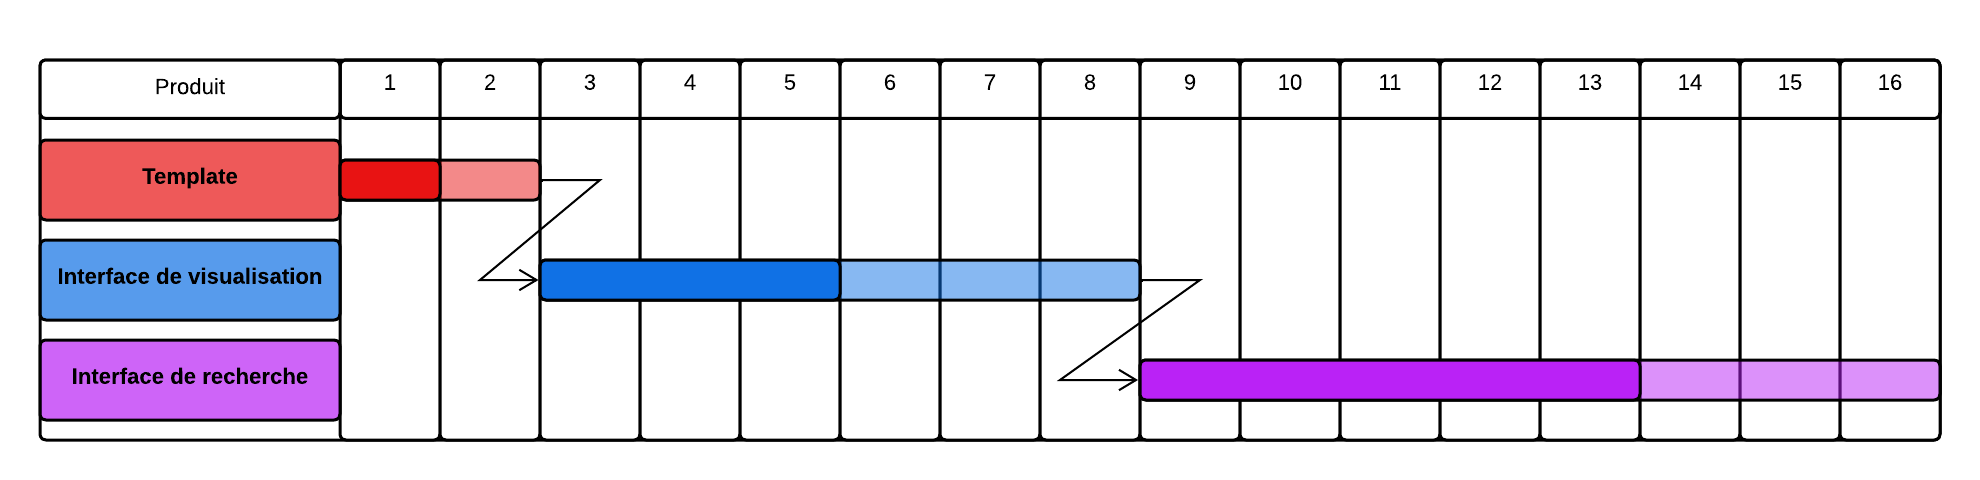
\includegraphics[scale=0.15]{Gantt}
            \end{center}
        \end{figure}
    \end{section}

    \begin{section}{Risques}
        \begin{subsection}{Retard sur jalon}
            Prévention : une estimation large des tâches sera effectuée pour éviter de mauvaise surprise pour le
            client.

            Risque d’occurrence : moyen.

            Niveau d’impact : moyen.

            Protocole en cas de déclenchement : la présentation des tâches est décalée d’un sprint. 
            Le planning est revu et le client prévenu.
        \end{subsection}

        \begin{subsection}{Absence temporaire d’un fournisseur}
            Prévention : puisque l’ensemble des développeurs ont concrètement les mêmes compétences, il est
            inutile de prévoir des chaînes de back-up.

            Risque d’occurrence : moyen.

            Niveau d’impact : moyen.

            Protocole en cas de déclenchement : les fournisseurs restants effectueront une réunion d’urgence pour déterminer 
            si les tâches assignées à l’absent dépassent leurs intervalles dans le planning. Si c’est le cas 
            une réallocation des tâches sera effectuée afin de limiter voire annuler les interblocages liés à 
            l’ordonnancement des tâches.

            Autrement rien ne change, les tâches seront seulement repoussées dans le planning.
        \end{subsection}

        \begin{subsection}{Absence définitive d’un fournisseurs}
            Prévention : puisque l’ensemble des développeurs ont concrètement les mêmes compétences, il est
            inutile de prévoir des chaînes de back-up.

            Risque d’occurrence : faible.

            Niveau d’impact : fort.

            Protocole en cas de déclenchement : les fournisseurs restants effectueront une réunion d’urgence pour réévaluer le 
            planning. Dans le cas où ce nouveau planning dépasserait la date de livraison, une réunion avec les clients sera 
            effectué pour les informer de la situation. Autrement le client sera juste notifié d’une modification de la 
            composition et recevra le nouveau planning.
        \end{subsection}

        \begin{subsection}{Absence temporaire d’un client principal}
            Prévention : mise en place d’une chaîne de back-up pour assurer le rôle de client principal.

            Risque d’occurrence : moyen.

            Niveau d’impact : moyen.

            Protocole en cas de déclenchement : les fournisseurs effectueront une réunion d’urgence pour évaluer si cette 
            absence modifie le planning, notamment au niveau des validations par le client.\\
            Toutes les communications et cérémonies seront redirigées vers un client secondaire désigné par le
            client principal. Dans le cas où il n’y a aucun client secondaire, les cérémonies ne seront pas
            assurées. Les communications seront mises en tampon. Le travail de l’équipe de fournisseurs continuera
            normalement jusqu’au jalon de validation qui seront reportés.
        \end{subsection}

        \begin{subsection}{Absence définitive d’un client}
            Prévention : s’assurer qu’il y ait plus d’un client principal.

            Risque d’occurrence : faible.

            Niveau d’impact : catastrophique.

            Protocole en cas de déclenchement : l’ensemble des communications et cérémonies se dérouleront avec le reste des 
            clients principaux.
            Dans le cas où tous les clients principaux sont indisponibles, le projet sera annulé faute de client.
            
        \end{subsection}

        \begin{subsection}{Manque de maîtrise d’un fournisseur sur VueJS}
            Prévention : formation à vuejs.

            Risque d’occurrence : faible.

            Niveau d’impact : moyen.

            Protocole en cas de déclenchement : l’équipe de fournisseurs effectuera une réunion d’urgence pour décider si le 
            manque est trop important ou non. Si ce n’est pas le cas les tâches du fournisseur défaillant seront revues pour 
            qu’il dispose de plus de temps afin qu’il puisse se documenter en même temps qu’il produit. Sinon, le fournisseur 
            défaillant passera en peer-programing.\\
            Quoi qu’il arrive le planning sera revu et le client informé de la situation.
        \end{subsection}

        \begin{subsection}{Perte de donnée}
            Prévention : utilisation d’un logiciel de gestion de version décentralisée.

            Risque d’occurence : faible.

            Niveau d’impact : fort.

            Protocole en cas de déclenchement : aucun, géré par la prévention.
        \end{subsection}
    \end{section}

    \begin{section}{Communication}
        Nous ne sommes pas en contact direct avec les contributeurs. La seule interaction se fera au travers
        de la documentation.

        L’ensemble des communications des fournisseurs se fera sur un serveur discord car ce dernier est
        facilement organisable. Ils effectueront des daily meetings permettant à chacun de savoir ce que fait
        l’autre.

        Le client sera informé du travail au travers de revues de backlog avec tous les fournisseurs, au
        travers du serveur discord FlopEDT! qui centralise déjà toutes les communications du projet. Ce
        discord sera également utilisé pour contacter les clients au besoin hors des cérémonies usuelles.

        L’utilisation d’un outil de version permettra aux différentes parties prenantes de suivre l’avancée du
        projet.
        
    \end{section}
\end{document}